%% Robust Representation Learning for Irregular Time Series under Observation-Process Shift
%% Draft v0.1 -- 2026-09-23. Built on the ACM sigconf template shipped in this folder.
%% Numbers marked [prelim] come from the current experimental budget (epoch cap 30 / patience 8, 2-3 seeds);
%% [RESULT NEEDED] marks experiments that are running or not yet run. Do not remove either marker without
%% replacing the underlying number.
\documentclass[sigconf,nonacm]{acmart}
\usepackage{booktabs}
\usepackage{multirow}
\usepackage{amsmath}
\usepackage{xcolor}
\newcommand{\todo}[1]{\textcolor{red}{[#1]}}
\newcommand{\prelim}{\textsuperscript{\dag}}

\AtBeginDocument{\providecommand\BibTeX{{Bib\TeX}}}
\settopmatter{printacmref=false}
\renewcommand\footnotetextcopyrightpermission[1]{}
\pagestyle{plain}

\begin{document}

\title{Robust Representation Learning for Irregular Time Series under Observation-Process Shift}

\author{Anonymous Authors}
\affiliation{\institution{Anonymous Institution}\country{}}

\begin{abstract}
Irregularly sampled multivariate time series arise whenever an underlying temporal process is recorded through a
measurement procedure that decides when, and which, variables are observed. Most learning methods for such data
focus on representing a given set of irregular observations. We study a different question: what happens when the
observation process itself changes between training and deployment, while the underlying temporal process stays
comparable? We formalize this \emph{observation-process shift} as a distinct source of distribution shift, and show
on a clinical forecasting benchmark that a strong query-based irregular encoder, trained on one observation
process, loses most of its accuracy when the same test trajectories are re-observed through a sparser, burstier,
or variable-specific process, even though its in-distribution error is unchanged. We then investigate three
mechanisms for robustness. (i)~\emph{Sampling-process augmentation}, which re-observes each training trajectory
through randomly drawn observation processes, reduces the relative error increase under shift from about 110\% to
about 15\% at no in-distribution cost and transfers to observation regimes never seen in training.
(ii)~An explicit representation-consistency objective between observation views, in contrast, adds nothing and
drives representations of different samples toward a common direction; observation-process robustness is not the
same as forcing representations to be identical across views. (iii)~\emph{Observation-aware query adaptation},
which conditions the encoder's aggregation queries on statistics of the observation pattern, recovers a substantial
part of the augmentation gain without any augmentation, with the gain traceable to observation-count statistics and
not to added capacity, but it is redundant once augmentation is used and can over-fit to training-time observation
statistics in classification. Finally, on a synthetic structural system with a known graph, we find that supplying
the correct variable-level structure as a soft attention prior is not distinguishable from supplying a shuffled or
an edge-free structure, which cautions against reading in-distribution gains from structural attention biases as
evidence of causal usefulness; only a hard constraint in a low-data regime separates correct from incorrect
structure, and a language-model-elicited physiological prior gives no benefit on real clinical data.
\todo{abstract numbers to be finalized with full-protocol multi-seed results}
\end{abstract}

\maketitle

\section{Introduction}
Many real-world temporal systems are observed irregularly. In intensive care, laboratory values are ordered when a
clinician decides they are needed; in environmental monitoring, sensors fail, are serviced, or report at
heterogeneous rates; in wearable sensing, contact loss and battery cycles create gaps. In all of these settings
the recorded data are not the underlying process but the outcome of two processes: the temporal dynamics of the
system and the \emph{observation process} that selects the times and variables at which the dynamics are seen.

A large body of work has developed encoders for such data, including recurrent models with decay
\cite{che2018grud}, continuous-time latent models \cite{rubanova2019latentode,debrouwer2019gruodebayes,kidger2020ncde},
set-function and attention-based aggregation \cite{horn2020seft,shukla2021mtand}, graph-guided models
\cite{zhang2022raindrop,zhang2024tpatchgnn}, and, most recently, query-based input embeddings that let standard
multivariate backbones consume irregular observations without interpolation \cite{lim2026quite}. These methods
differ in how they represent a given set of irregular observations, and are typically evaluated under the
observation process of the benchmark on which they are trained.

This paper asks a complementary question. The observation process is not a fixed property of a domain: a
different hospital orders labs on a different schedule, a sensor network is redeployed with a different sampling
policy, a device firmware update changes when readings are logged. In each case the underlying dynamics are
comparable but the observation process has shifted. Does a representation learned under one observation process
remain useful under another?

We make the distinction explicit (Section~\ref{sec:problem}): the observed sample is $\mathcal O=\mathcal S(X)$,
where $X$ is the underlying trajectory and $\mathcal S$ is drawn from an observation-process distribution
$P_{\mathrm{obs}}$. \emph{Process shift} changes the distribution of $X$; \emph{observation-process shift} changes
$P_{\mathrm{obs}}$ while $X$ stays comparable. We study the second setting, which is largely invisible to standard
benchmark protocols because training and test data are drawn from the same $P_{\mathrm{obs}}$.

Our first finding is that the phenomenon is real and large. On PhysioNet-2012 forecasting
\cite{silva2012physionet}, a query-based irregular encoder on an inverted-Transformer backbone reaches a test MSE
of $0.0054$ under the training observation process, but when the \emph{same} test trajectories are re-observed with
70\% of the observations dropped at random, with 30\% of the variables unobserved, or with a systematic
subsampling regime absent from training, the error roughly triples (Section~\ref{sec:phenomenon}). The degradation
is not explained by observation count alone: two regimes with the same density can have very different effects.

We then investigate three hypotheses about how representation learning should account for the observation
process, treating them as independent rather than as components of one model:

\begin{itemize}
\item \textbf{Q1 (sampling invariance).} Training the encoder on multiple randomly drawn observation views of each
trajectory (\emph{sampling-process augmentation}) reduces the relative degradation under shift from $+111\%$ to
$+15\%$ at no in-distribution cost, and transfers to regimes never seen in training. An explicit
representation-consistency term between views, however, brings no additional robustness and pushes
representations of \emph{different} samples toward a common direction (Section~\ref{sec:aug}). We report this
negative result because it separates two ideas that are often conflated: robustness to the observation process
and invariance of the representation.
\item \textbf{Q2 (observation-aware adaptation).} Conditioning the encoder's aggregation queries on statistics of
the observation pattern seen by each query (\emph{observation-aware queries}) halves the error under
variable-specific shift without any augmentation, with the gain attributable to count-based density statistics
rather than to added parameters (Section~\ref{sec:adaptive}). The two mechanisms overlap rather than stack.
\item \textbf{Q3 (structural prior).} On a synthetic structural system with a known graph, a soft attention
bias built from the oracle graph gives at most a small in-distribution gain that a \emph{shuffled} graph and an
edge-free identity bias reproduce, and no advantage when the target's causes are removed. Only when data are
scarce (900 trajectories) and the structure is imposed as a hard constraint does the correct graph separate from
every wrong graph of the same shape, on all seeds. A physiological prior elicited from a language model gives no
benefit on PhysioNet at any strength (Section~\ref{sec:structure}).
\end{itemize}

We use a query-based irregular encoder \cite{lim2026quite} as the experimental substrate throughout because it
consumes irregular observations natively and exposes a natural point (the aggregation query) at which to condition
on the observation process. Nothing in the formulation or the mechanisms depends on this particular encoder.

\paragraph{Contributions.}
(1)~We distinguish observation-process shift from process shift and establish it empirically as a large,
density-independent source of degradation for irregular time-series encoders.
(2)~We show that sampling-process augmentation provides most of the available robustness, transfers to unseen
regimes, and that explicit cross-view representation consistency is neither necessary nor sufficient.
(3)~We study observation-aware query adaptation as a mechanism that recovers robustness without augmentation and
characterize which observation statistics carry the effect.
(4)~We provide a controlled study of structural attention priors under irregular observation, with shuffled and
random controls, and find that in-distribution gains do not certify structural usefulness.

\section{Related Work}
\paragraph{Irregular multivariate time-series learning.}
Interpolation-based approaches map irregular observations to a regular grid before encoding
\cite{shukla2019ipn}; continuous-time approaches evolve a latent state between observations with differential
equations \cite{rubanova2019latentode,debrouwer2019gruodebayes,kidger2020ncde}; set-based approaches treat
observations as an unordered set and aggregate with attention \cite{horn2020seft,shukla2021mtand};
graph-based approaches model inter-variable dependencies explicitly \cite{zhang2022raindrop,zhang2024tpatchgnn}.
Query-based embeddings \cite{lim2026quite} aggregate the observations belonging to a variable or a temporal patch
into a fixed-size token through masked attention with a learnable query, so that standard multivariate backbones
\cite{liu2024itransformer,nie2023patchtst} can be used unchanged. Our work does not propose a new encoder; it asks
how any such encoder behaves when the observation process changes.

\paragraph{Missingness and observation processes.}
The statistical missing-data literature distinguishes mechanisms by their dependence on observed and unobserved
values \cite{rubin1976missing}; in clinical data, the pattern of missingness is itself informative
\cite{lipton2016informative,che2018grud}. Most learning work treats irregularity as a property of the dataset
and evaluates robustness by varying a missingness \emph{rate}. We instead vary the observation \emph{process}
(random, bursty, variable-specific, systematically subsampled) at fixed or comparable density, and study the case
in which the process differs between training and test.

\paragraph{Robust and invariant representation learning.}
Augmentation-based robustness \cite{tobin2017domainrand,wen2021augmentation} and invariance objectives
\cite{arjovsky2019irm} address distribution shift by exposing a model to, or enforcing constancy across,
environments. Cross-view consistency and contrastive objectives \cite{chen2020simclr,grill2020byol} are known to
require mechanisms that prevent collapse; variance-preserving formulations \cite{bardes2022vicreg} make this
explicit. Our observation views are a form of environment randomization applied to the measurement process
rather than to the signal, and our negative result on cosine consistency is consistent with the collapse
literature.

\paragraph{Structural and causal time-series learning.}
Granger causality \cite{granger1969} and its neural and constraint-based extensions
\cite{tank2021neuralgranger,runge2019pcmci} identify predictive temporal dependencies; continuous structure
learning \cite{zheng2018notears} recovers acyclic graphs. We do not perform discovery: we ask whether externally
supplied structure, used as an attention prior \cite{vaswani2017attention}, helps under irregular observation, and
we control for the effect of the prior's mere presence.

\paragraph{Adaptive and conditional representations.}
Feature-wise conditioning \cite{perez2018film} adapts computation to side information. Observation-aware queries
apply this idea to the aggregation step of an irregular encoder, with the side information being a summary of the
observation process itself.

\section{Learning under Observation-Process Shift}
\label{sec:problem}
\subsection{Problem formulation}
Let $X=\{x(t)\}_{t\in\mathcal T}$, $x(t)\in\mathbb R^N$, be an underlying multivariate temporal process. The
learner never observes $X$ directly. It receives a finite set of timestamped, partially observed measurements
\begin{equation}
\mathcal O=\{(t_k, x(t_k), m_k)\}_{k=1}^{K},\qquad m_k\in\{0,1\}^N,
\end{equation}
where $m_k$ indicates which variables were measured at time $t_k$. We model the selection of $\{(t_k,m_k)\}$ as an
\emph{observation process} $\mathcal S\sim P_{\mathrm{obs}}$ and write $\mathcal O=\mathcal S(X)$. A training set is
drawn from a joint distribution over $(X,\mathcal S)$; a model $f$ maps $\mathcal O$ to a representation
$z(\mathcal O)$ and then to a task output (a forecast of $x$ over a future window, or a label).

We distinguish two shifts between training and deployment: \emph{process shift}, in which $P(X)$ changes, and
\emph{observation-process shift}, in which $P_{\mathrm{obs}}$ changes while $P(X)$ is comparable. This paper
concerns the latter. Two datasets can contain observations of the same underlying process while differing in
observation density, in the temporal clustering of observations, in which variables are observed, or in the
regularity of the sampling. Standard evaluation, which draws training and test data from the same
$P_{\mathrm{obs}}$, cannot detect sensitivity to this shift.

\paragraph{Evaluation protocol.}
Given a trained model and a test set drawn under the training observation process, we re-observe the test
inputs through a different process $\mathcal S'$ and keep the prediction targets unchanged. For a metric
$\mathrm{MSE}$ we report the in-distribution value $\mathrm{MSE}_{\mathrm{ID}}$ (original observations) and the
out-of-distribution value $\mathrm{MSE}_{\mathcal S'}$, and summarize robustness by the relative degradation
\begin{equation}
\Delta_{\mathrm{shift}}=\frac{\overline{\mathrm{MSE}_{\mathcal S'}}-\mathrm{MSE}_{\mathrm{ID}}}{\mathrm{MSE}_{\mathrm{ID}}},
\end{equation}
averaged over a set of shifted processes $\mathcal S'$. We use four families of $\mathcal S'$, each of which only
edits the observation mask and never introduces artificial values: \textbf{random} (each observation dropped
independently with probability $p$), \textbf{bursty} (two contiguous time windows covering a fraction $p$ of the
observed range are removed), \textbf{variable-specific} (each variable removed entirely with probability $p$), and
\textbf{stride} (every $k$-th observation of each variable is kept, giving a lower but regular sampling rate).
When a model is trained with a mixture of processes, the \emph{unseen} regimes are those absent from the mixture
(here: variable removal at $p=0.5$ and the stride family).

\subsection{Sampling-process augmentation}
\label{sec:method-aug}
The first mechanism treats the observation process as a source of nuisance variation to be randomized over. For
each training trajectory we draw $V$ observation processes $\mathcal S_1,\dots,\mathcal S_V$ from a mixture
$P_{\mathrm{mix}}$ and train on all $V$ views:
\begin{equation}
\mathcal L=\frac1V\sum_{v=1}^{V}\mathcal L_{\mathrm{task}}\big(f(\mathcal S_v(X)),\,y\big)
\;+\;\lambda\,\mathcal L_{\mathrm{cons}}\big(z(\mathcal S_1(X)),\,z(\mathcal S_2(X))\big).
\label{eq:aug}
\end{equation}
With $\lambda=0$ this is augmentation only. The consistency term, $\mathcal L_{\mathrm{cons}}=1-\cos(z_1,z_2)$ on
the encoder output (or a mean-squared distance between the two views' predictions), encodes the hypothesis that
two observations of the same trajectory should map to the same representation. We emphasize that the desired
property is \emph{observation-process} invariance: $z(\mathcal S_1(X))\approx z(\mathcal S_2(X))$ for the same
$X$, while $z(X_a)\neq z(X_b)$ for trajectories that differ in task-relevant ways. Whether a cross-view objective
achieves the first without violating the second is an empirical question, and we monitor it directly with
between-sample similarity diagnostics (Section~\ref{sec:aug}).

\subsection{Observation-aware representation}
\label{sec:method-adaptive}
A query-based irregular encoder aggregates the observations of a target (a variable, or a variable within a
temporal patch) through masked attention from a learnable query token $q_i$. The query is the same for every
sample, regardless of how many observations it will aggregate or how they are spaced. The second mechanism makes
the query a function of the observation pattern:
\begin{equation}
q_i(\mathcal O)=q_i^{\mathrm{base}}+g_\theta\big(s_i(\mathcal O)\big),
\end{equation}
where $s_i(\mathcal O)\in\mathbb R^7$ summarizes the observations available to query $i$: the log observation
count and the count normalized by the maximum length (\emph{density}); the mean and standard deviation of the
inter-observation gaps and the observed time span (\emph{gap timing}); an indicator that any observation is
present and the fraction of targets in the same sample that have observations (\emph{availability}). $g_\theta$ is
a two-layer MLP whose output layer is zero-initialized, so every adaptive variant starts exactly at the
non-adaptive encoder, and the added parameters are $3.6\%$ of the base model. The hypothesis is not that more
parameters help, but that the optimal aggregation of a sparse, clustered, or variable-depleted observation set
differs from that of a dense one, and that the encoder can only adjust if it is told which case it is in. We test
this against a control in which $g_\theta$ receives Gaussian noise of the same dimension.

\subsection{Structural priors}
\label{sec:method-structure}
The third mechanism supplies variable-level structure to the cross-variable attention of the backbone. Let
$M\in\{0,1\}^{N\times N}$ with $M_{ij}=1$ if variable $j$ influences variable $i$ (and $M_{ii}=1$). The attention
of variable token $i$ over variable tokens $j$ becomes
\begin{equation}
A_{ij}=\operatorname{softmax}_j\!\left(\frac{Q_iK_j^{\top}}{\sqrt d}+\lambda M_{ij}\right),
\end{equation}
a soft bias toward attending to a variable's presumed causes. We also consider a hard mask (attend only where
$M_{ij}=1$) and a free learned $N\times N$ bias (no structure supplied). We distinguish three sources of $M$: an
\emph{oracle} graph, known because it generated the data; an \emph{externally supplied} prior, such as a
domain-knowledge graph written for a real dataset; and \emph{arbitrary} structure used as a control (identity,
random edges with the same count, a variable-shuffled version of the oracle graph, and a noisy version with a
fraction of entries flipped). An attention matrix does not become causal by being placed inside attention; the
controls are what allow any gain to be attributed to the structure rather than to the presence of a bias.

\section{Experimental Setup}
\label{sec:setup}
\paragraph{Datasets and tasks.}
\emph{PhysioNet-2012} \cite{silva2012physionet}: 12{,}000 ICU stays, 41 variables, 24-hour history to 24-hour
forecast, following the t-PatchGNN protocol \cite{zhang2024tpatchgnn} (60/20/20 split, min-max normalization,
masked MSE/MAE on observed targets). \emph{P12 classification}: in-hospital mortality on the same source with the
Raindrop preprocessing and splits \cite{zhang2022raindrop} (AUROC, AUPRC; a single split in the current budget).
\emph{Synthetic structural system} (Section~\ref{sec:structure}): 10 abstract channels driven by a known directed
graph, 4{,}000 trajectories over a 48-unit window, each channel observed with a channel-specific probability in
$[0.2,0.4]$.

\paragraph{Base encoder and backbones.}
We use the query-based irregular embedding of \cite{lim2026quite} with an inverted-Transformer backbone
\cite{liu2024itransformer} for forecasting (hidden size 64, 4 heads, 3 layers, patch length 6) and a PatchTST
backbone \cite{nie2023patchtst} for classification, following the published per-backbone settings. All models are
trained with Adam (learning rate $10^{-3}$, batch 32) with early stopping on validation loss. The current budget
uses an epoch cap of 30 and patience 8 on PhysioNet and a cap of 100 on the synthetic data; the published protocol
uses patience 50, and we mark all numbers obtained under the reduced budget with~\prelim. \todo{replace with
full-protocol, 5-seed runs before submission}

\paragraph{Observation views.}
The training mixture $P_{\mathrm{mix}}$ draws uniformly from random dropout at $p\in\{0.3,0.6\}$, bursty removal
at $p\in\{0.3,0.5\}$, and variable removal at $p=0.3$. Evaluation uses these plus random $p=0.5$ and $0.7$, and the
unseen regimes variable $p=0.5$, stride 2 and stride 3. All evaluation views use a fixed random seed so that every
model sees the same re-observed test set.

\paragraph{Cost.}
We report parameter count, training time per epoch, peak GPU memory and inference time per series, measured on
one 8\,GB laptop GPU.

\section{Does Observation-Process Shift Matter?}
\label{sec:phenomenon}
Table~\ref{tab:phenomenon} and Figure~\ref{fig:robustness} (blue bars) show the base encoder trained under the
PhysioNet observation process and tested on the same trajectories under other processes. In distribution it
reaches an MSE of $0.0054\pm0.0001$ over three seeds, comparable to the published result. Under shift the error
grows by a factor of two to four: $0.0164$ with 70\% random dropout, $0.0166$ with 30\% of variables removed,
$0.0225$ with 50\% removed, and $0.0108$ under stride-3 subsampling. Averaged over the six standard shifted views,
$\Delta_{\mathrm{shift}}=+111\%\pm8\%$.

Three observations follow. First, the degradation is not a function of density alone: bursty removal of 50\% of
the observed range ($0.0079$) costs far less than random removal of 50\% of the points ($0.0119$), and stride-2
subsampling, which halves the observation count like random $p=0.5$, costs $0.0091$. The temporal structure of what
is missing matters as much as how much is missing. Second, variable-specific shift is the most damaging: losing
30\% of the variables entirely costs as much as losing 70\% of all points. Third, the encoder without the
irregular embedding (a vanilla inverted Transformer with a time-agnostic input layer) is worse everywhere
($0.0178$ in distribution) but degrades by a similar factor, so the sensitivity is not an artifact of the
query-based embedding. Observation-process shift is therefore a real and large failure mode that standard
evaluation does not reveal.

\begin{table}[t]
\caption{Observation-process shift on PhysioNet forecasting (test MSE, mean~$\pm$~std over seeds). The base
encoder is trained once; test inputs are re-observed through each process, targets unchanged. Regimes marked $^*$
never occur in the augmentation mixture. \prelim: reduced training budget.}
\label{tab:phenomenon}
\small
\begin{tabular}{lcccccc}
\toprule
Model & ID & random .7 & bursty .5 & variable .3 & variable .5$^*$ & stride 3$^*$ \\
\midrule
vanilla backbone (no irregular emb.)\prelim & 0.0178 & 0.0347 & 0.0229 & 0.0416 & 0.0557 & 0.0208 \\
query-based irregular encoder\prelim & 0.0054$\pm$.0001 & 0.0164$\pm$.0011 & 0.0079$\pm$.0002 & 0.0166$\pm$.0015 & 0.0225$\pm$.0023 & 0.0108$\pm$.0006 \\
\bottomrule
\end{tabular}
\end{table}

\begin{figure}[t]
\centering
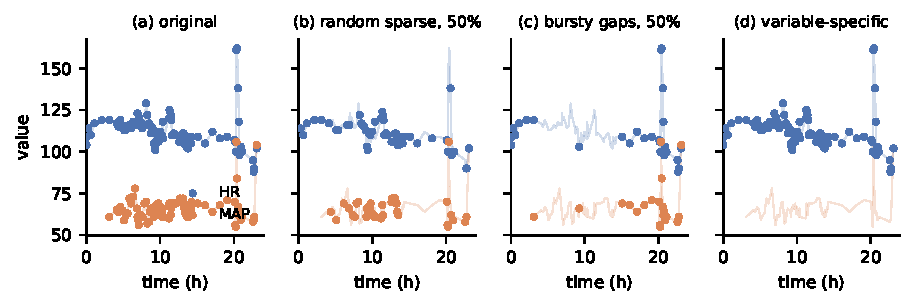
\includegraphics[width=\linewidth]{figures/fig1_observation_shift.pdf}
\caption{The same ICU stay (heart rate and mean arterial pressure over 24\,h) under four observation processes.
Faint lines connect the original observations; markers show what the model receives. (b)--(d) are the evaluation
views used throughout: the underlying trajectory is identical, only the observation process differs.}
\label{fig:views}
\end{figure}

\section{Sampling-Process Augmentation}
\label{sec:aug}
\paragraph{Augmentation removes most of the degradation.}
Training with two mixture-drawn views per batch and $\lambda=0$ (augmentation only) leaves the in-distribution
error unchanged ($0.0054\pm0.0001$) and reduces every shifted error to within 30\% of it (Table~\ref{tab:aug},
Figure~\ref{fig:robustness}): random 70\% dropout $0.0070$, variable 30\% $0.0068$, and $\Delta_{\mathrm{shift}}$
falls from $+111\%$ to $+15\%\pm1\%$. The effect is identical on both seeds to within $10^{-4}$. It also transfers
to regimes absent from the mixture: variable removal at 50\% ($0.0075$ vs.\ $0.0225$) and stride subsampling
($0.0057$ vs.\ $0.0108$), a regime \emph{type} the model never saw. Under the same budget on P12 classification
the augmented model is better in distribution (AUROC $85.5$ vs.\ $83.7$) and under every shift
(Table~\ref{tab:cls}).

\paragraph{A mixture of regimes is needed for transfer.}
Training on a single regime protects that regime and its neighbours but not the others: random-dropout-only
training leaves variable removal at $0.0087$; bursty-only training leaves random 70\% at $0.0080$ and variable
removal at $0.0101$ (Table~\ref{tab:aug}). Transfer to an unseen regime is a property of the diversity of the
training mixture, not of augmentation per se.

\paragraph{Explicit consistency adds nothing and moves representations toward a common direction.}
Adding the cosine consistency term at $\lambda\in\{0.01,0.1,1\}$, or a prediction-level consistency term, changes
no shifted error by more than the seed spread and slightly worsens in-distribution error at $\lambda=1$
($0.0059$; Figure~\ref{fig:consistency}). The diagnostics in Table~\ref{tab:collapse} show why. Augmentation alone
yields a cosine of $0.90$ between the two views of the same sample and $0.81$ between views of \emph{different}
samples. The representation-level consistency term raises both to $0.99$--$1.00$ and reduces the per-feature
standard deviation over the batch from $0.41$ to $0.02$--$0.11$: the objective is satisfied by aligning every
sample's representation to a shared direction, not by making the two views of a sample agree while keeping
samples apart. The task loss preserves enough residual variance for the decoder, which is why the forecasting
error barely moves, but the term does not achieve observation-process invariance in the intended sense.
Prediction-level consistency does not exhibit this behaviour and is equally ineffective. We conclude that
observation-process robustness is obtained from exposure to varied observation processes and is not equivalent
to enforcing representation identity across views; an invariance objective that is to add anything would need
an explicit variance-preserving term \cite{bardes2022vicreg}.

\begin{table}[t]
\caption{Sampling-process augmentation on PhysioNet forecasting (test MSE\prelim). Main rows: 2 seeds; ablations:
seed 1. $\Delta_{\mathrm{shift}}$ averages the six standard shifted views.}
\label{tab:aug}
\small
\begin{tabular}{lcccccc}
\toprule
Training & ID & random .7 & variable .3 & variable .5$^*$ & stride 3$^*$ & $\Delta_{\mathrm{shift}}$ \\
\midrule
none (base encoder) & 0.0054 & 0.0164 & 0.0166 & 0.0225 & 0.0108 & $+111\%$ \\
mixed views, $\lambda=0$ & \textbf{0.0054} & \textbf{0.0070} & \textbf{0.0068} & \textbf{0.0075} & \textbf{0.0057} & $+15\%$ \\
mixed views, cosine $\lambda=0.1$ & 0.0056 & 0.0071 & 0.0070 & -- & -- & $+14\%$ \\
\midrule
mixed views, cosine $\lambda=0.01$ & 0.0056 & 0.0073 & 0.0070 & -- & -- & $+15\%$ \\
mixed views, cosine $\lambda=1$ & 0.0059 & 0.0074 & 0.0072 & -- & -- & $+13\%$ \\
mixed views, prediction consistency $\lambda=0.1$ & 0.0057 & 0.0070 & 0.0068 & 0.0076 & 0.0058 & $+11\%$ \\
random .5 only, $\lambda=0.1$ & 0.0059 & 0.0073 & 0.0087 & -- & -- & $+15\%$ \\
bursty .5 only, $\lambda=0.1$ & 0.0057 & 0.0080 & 0.0101 & -- & -- & $+26\%$ \\
\bottomrule
\end{tabular}
\end{table}

\begin{table}[t]
\caption{Representation diagnostics (last three epochs, seed 1): cosine between the two views of the same
sample (pos.), between views of different samples (neg.), and per-feature standard deviation over the batch.}
\label{tab:collapse}
\small
\begin{tabular}{lccc}
\toprule
Training & pos.\ cos & neg.\ cos & feature std \\
\midrule
mixed views, $\lambda=0$ & 0.896 & 0.807 & 0.413 \\
prediction consistency, $\lambda=0.1$ & 0.909 & 0.836 & 0.377 \\
representation consistency, $\lambda=0.01$ & 0.996 & 0.992 & 0.113 \\
representation consistency, $\lambda=0.1$ & 1.000 & 0.999 & 0.044 \\
representation consistency, $\lambda=1$ & 1.000 & 1.000 & 0.018 \\
\bottomrule
\end{tabular}
\end{table}

\begin{figure}[t]
\centering
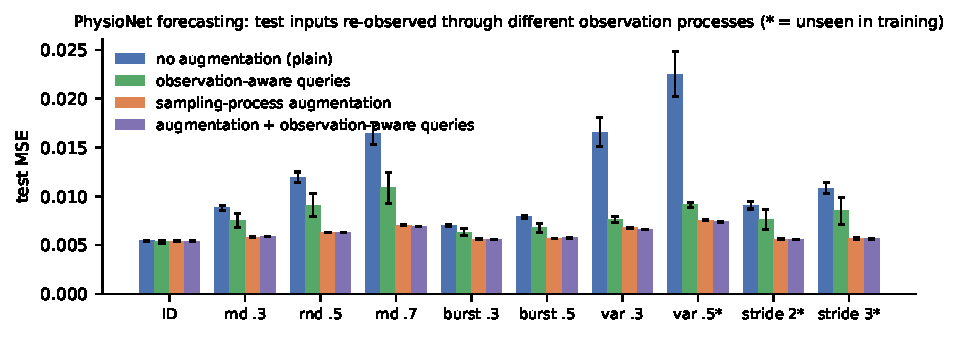
\includegraphics[width=\linewidth]{figures/fig3_robustness.pdf}
\caption{Test MSE on PhysioNet when the test inputs are re-observed through different processes (mean $\pm$ std
over seeds). Regimes marked $^*$ do not occur in the training mixture.}
\label{fig:robustness}
\end{figure}

\begin{figure}[t]
\centering
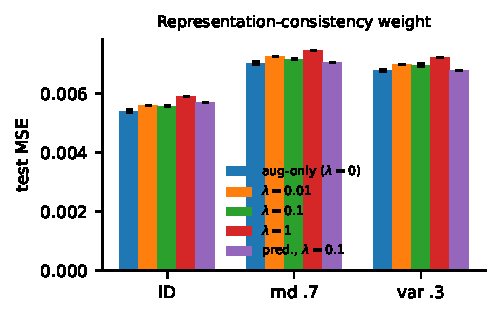
\includegraphics[width=0.6\linewidth]{figures/fig3b_consistency.pdf}
\caption{Cross-view consistency weight. No setting improves on augmentation alone.}
\label{fig:consistency}
\end{figure}

\section{Observation-Aware Representation}
\label{sec:adaptive}
\paragraph{Without augmentation, observation-aware queries recover part of the robustness.}
Table~\ref{tab:adaptive} compares the base encoder with the observation-aware variant under standard training.
Over two seeds the in-distribution error is unchanged ($0.0053$ vs.\ $0.0054$), the error under variable removal
halves ($0.0076$ vs.\ $0.0166$ at 30\%; $0.0091$ vs.\ $0.0225$ at 50\%, an unseen severity), and the errors under
random dropout and stride subsampling decrease by a seed-dependent amount ($0.0109$ vs.\ $0.0164$; $0.0085$ vs.\
$0.0108$; large on one seed, small on the other). The variable-removal effect is consistent across seeds; the
others are suggestive and require more seeds.

\paragraph{The effect is due to the observation information, not to capacity.}
The noise-fed control, which has the same MLP and receives Gaussian noise instead of $s_i(\mathcal O)$, stays
close to the base encoder on every view (random 70\%: $0.0146$ vs.\ $0.0170$; stride unchanged), with a modest
gain under variable removal ($0.0137$ vs.\ $0.0187$) that we attribute to the noise acting as a regularizer on
the query. Every informative variant is clearly better than this control.

\paragraph{Which statistics matter.}
Density statistics alone (log count and count per length) recover about 90\% of the full-statistics gain
($0.0103$ / $0.0075$ / $0.0080$ on random 70\% / variable 30\% / stride 3, vs.\ $0.0093$ / $0.0073$ / $0.0071$
for all statistics). Availability alone captures the variable-removal gain ($0.0082$) but less of the dropout
gain ($0.0130$). Gap-timing statistics alone are ineffective ($0.0151$ / $0.0146$ / $0.0109$). The query benefits
from knowing \emph{how much} it will aggregate, not \emph{when} the observations fall.

\paragraph{Adaptation and augmentation overlap rather than stack.}
Under mixed-view training the observation-aware model is within $0.0002$ MSE of augmentation alone on every view
(Table~\ref{tab:adaptive}, last rows) and within $0.3$ AUROC on P12 (Table~\ref{tab:cls}). When augmentation is
available the adaptation is redundant; when it is not, adaptation recovers roughly half of the augmentation gain.

\paragraph{A failure case.}
On P12 classification without augmentation, the observation-aware model improves in-distribution AUROC
($85.2$ vs.\ $83.7$) and holds under stride subsampling, but is \emph{worse} than the base encoder under random
dropout ($76.9$ vs.\ $81.6$) and variable removal ($77.4$ vs.\ $79.6$): the classifier learns to rely on the
training-time distribution of observation statistics and extrapolates poorly when it shifts. With mixed-view
training the problem disappears and the combination is the best P12 configuration ($86.2$ AUROC in distribution,
$83.9$ under 70\% dropout). Observation-aware adaptation therefore requires the training data to cover varied
observation regimes; it is not a substitute for that coverage.

\begin{table}[t]
\caption{Observation-aware queries on PhysioNet forecasting (test MSE\prelim). Standard training unless noted;
2 seeds for the main rows, seed 1 for ablations.}
\label{tab:adaptive}
\small
\begin{tabular}{lccccc}
\toprule
Query & ID & random .7 & variable .3 & variable .5$^*$ & stride 3$^*$ \\
\midrule
fixed (base encoder), 3 seeds & 0.0054 & 0.0164 & 0.0166 & 0.0225 & 0.0108 \\
observation-aware, all statistics & \textbf{0.0053} & 0.0109 & \textbf{0.0076} & \textbf{0.0091} & 0.0085 \\
\midrule
noise-fed control (seed 1) & 0.0055 & 0.0146 & 0.0137 & 0.0178 & 0.0107 \\
density only (seed 1) & 0.0053 & 0.0103 & 0.0075 & 0.0089 & 0.0080 \\
availability only (seed 1) & 0.0054 & 0.0130 & 0.0082 & 0.0098 & 0.0092 \\
gap timing only (seed 1) & 0.0055 & 0.0151 & 0.0146 & 0.0199 & 0.0109 \\
\midrule
mixed views, fixed query & 0.0054 & 0.0070 & 0.0068 & 0.0075 & 0.0057 \\
mixed views, observation-aware & 0.0054 & 0.0069 & 0.0066 & 0.0074 & 0.0056 \\
\bottomrule
\end{tabular}
\end{table}

\begin{table}[t]
\caption{P12 in-hospital mortality (AUROC / AUPRC, Raindrop split 1\prelim).}
\label{tab:cls}
\small
\begin{tabular}{lcccc}
\toprule
Training & ID & random .7 & variable .3 & stride 3$^*$ \\
\midrule
base encoder & 83.7 / 47.3 & 81.6 / 40.4 & 79.6 / 36.8 & 83.7 / 47.6 \\
observation-aware queries & 85.2 / 48.6 & 76.9 / 32.4 & 77.4 / 36.0 & 84.6 / 47.6 \\
mixed views & 85.5 / 49.7 & 84.0 / 43.1 & 81.5 / 39.8 & 85.7 / 49.6 \\
mixed views + cosine consistency & 85.5 / 48.4 & 84.2 / 43.8 & 81.6 / 39.0 & 85.7 / 48.7 \\
mixed views + observation-aware & \textbf{86.2} / 49.5 & 83.9 / 42.1 & 81.4 / 40.0 & \textbf{86.1} / \textbf{50.1} \\
\bottomrule
\end{tabular}
\end{table}

\section{Structural Priors}
\label{sec:structure}
\paragraph{Synthetic structural system.}
We simulate 10 channels on a 48-unit window with step $0.5$. Root channels ($0,4,5,7,9$) follow a damped
oscillator with a sample-specific frequency and phase; every other channel $i$ follows
$x_i(t+1)=0.5\,x_i(t)+0.9\sum_{j\to i}\tanh x_j(t)+\epsilon$, with edges $0\to1\to2$, $0\to3$, $4\to2$, $5\to6$,
$7\to8$ and channel $9$ isolated (Figure~\ref{fig:structure}, left). Channel $2$ is the target $Y$: its parents are
$1$ and $4$, its only grand-parent is $0$, and channels $5$--$9$ cannot influence it. Each channel is observed at
each step with a channel-specific probability in $[0.2,0.4]$. The channels are abstract; the graph plays two
roles that we keep separate: it generates the data, and it may be supplied to the model as an oracle prior.

\paragraph{The base encoder uses the structure.}
Removing $Y$'s five non-causal channels from the test inputs leaves the error on $Y$ unchanged ($0.0279$ vs.\
$0.0273$), whereas removing its two parents raises it to $0.0437$ and removing its grand-parent and a sibling to
$0.0368$ (Figure~\ref{fig:structure}, right). The encoder has learned which channels matter for $Y$ from data
alone, which is the precondition for asking whether a supplied graph helps.

\paragraph{With ample data, a soft oracle prior is not distinguishable from a shuffled one.}
Table~\ref{tab:structure} reports the full-data results (2{,}400 training trajectories) over three seeds\prelim.
The oracle soft bias at $\lambda=2$ is within seed noise of no bias on all channels ($0.0192\pm0.0020$ vs.\
$0.0198\pm0.0006$) and on $Y$ ($0.0256$ vs.\ $0.0267$); a shuffled graph, in which the same edges connect the
wrong channels, gives the same numbers ($0.0191\pm0.0011$); an identity bias with no edges at all reproduces the
oracle's best seed exactly ($0.0172$ vs.\ $0.0172$ overall); and a dense noisy graph erases the effect. The
$\lambda$ sweep is non-monotone. On the discriminative test, removal of $Y$'s parents, no soft-biased model is
better than the base encoder, and the oracle-biased model is the worst ($0.0531$ vs.\ $0.0474$) and the least
robust to random dropout ($0.1150$ vs.\ $0.1005$). The small in-distribution effect of a sparse soft bias is
therefore a regularization effect that any sparse bias produces, not a use of the structure. The shuffled and
identity controls are the important ones: an in-distribution improvement from a ``causal'' attention bias is not
evidence that the structure is being used. The hard mask with the oracle graph behaves like the identity bias in
distribution ($0.0177$, seed~1) but makes $Y$ depend strongly on its parents ($0.0781$ when removed), and the free
learned bias is indistinguishable from no bias.

\paragraph{With scarce data, a hard oracle constraint helps and every wrong constraint hurts.}
With 900 training trajectories (Table~\ref{tab:lowdata}), the soft biases remain inert, but a hard mask that
restricts each variable's attention to its true causes is the best configuration on every seed (overall
$0.0287\pm0.0022$; $Y$ $0.0370$), about 14\% below the same hard mask built from a shuffled, identity or random
graph ($0.0331$--$0.0340$; $Y\approx0.050$) and below the unconstrained encoder. Its $Y$ error is unchanged when
the non-causal channels are removed and it is the only configuration whose $Y$ error rises when $Y$'s parents are
removed ($0.0714$); every wrong-structure mask leaves $Y$ at about $0.050$ on every view, i.e.\ $Y$ is then
predicted from its own observations alone. This is the one result in our structural experiments where correct
structure separates from incorrect structure of the same shape in the direction the hypothesis predicts, and it
survives the shuffled, identity and random controls. It is confined to the hard constraint and to the low-data
regime, and it costs robustness to random dropout ($0.101$ vs.\ $0.083$--$0.092$ for the wrong masks) because the
constrained model relies on fewer channels. We also note an optimization effect: with either bias, a fraction of
seeds stalled on a constant-predictor plateau under standard early stopping and required a minimum-epoch guard
(Section~\ref{sec:analysis}).

\paragraph{Real data with an externally supplied prior.}
For PhysioNet we wrote a sparse physiological prior over the 41 variables (58 directed edges, e.g.\ mechanical
ventilation $\to$ FiO$_2$ $\to$ PaO$_2$, urine output $\to$ creatinine, PaCO$_2$ $\to$ pH). Following the
distinction above, this is a \emph{semantic prior} elicited from a language model from variable names and
textbook physiology, not a validated causal graph, and its value is tested against shuffled and random versions
of itself. Table~\ref{tab:physprior} shows that no use of it improves on the base encoder: in-distribution error is
unchanged for every variant ($0.0053$--$0.0057$ vs.\ $0.0054$), every soft prior is \emph{less} robust under
random dropout and variable removal at $\lambda\in\{1,2\}$, and the shuffled prior behaves like the real one. The
hard mask reduces the damage from variable removal ($0.0149$ vs.\ $0.0166$), but a random prior with the same
edge count reduces it equally ($0.0150$), so the effect is that of restricting cross-variable attention, not of the
physiology. A free learned bias is indistinguishable from no bias. On this dataset, therefore, the semantic prior
does not compensate for the absence of an estimated graph; whether the prior is poor or the benchmark leaves no
room for it cannot be separated without a validated clinical graph.

\begin{table}[t]
\caption{Language-model-elicited physiological prior on PhysioNet forecasting (test MSE\prelim; 3 seeds for the
base encoder, 2 for the $\lambda=2$ rows, 1 otherwise).}
\label{tab:physprior}
\small
\begin{tabular}{lcccccc}
\toprule
Prior in variable attention & ID & random .7 & bursty .5 & variable .3 & variable .5$^*$ & stride 3$^*$ \\
\midrule
none (base encoder) & 0.0054 & \textbf{0.0164} & 0.0079 & 0.0166 & 0.0225 & 0.0108 \\
semantic prior, soft $\lambda=1$ & \textbf{0.0053} & 0.0178 & 0.0082 & 0.0194 & 0.0277 & 0.0101 \\
semantic prior, soft $\lambda=2$ & 0.0055 & 0.0185 & 0.0085 & 0.0213 & 0.0304 & 0.0111 \\
semantic prior, soft $\lambda=5$ & 0.0057 & 0.0196 & 0.0088 & 0.0156 & 0.0230 & 0.0124 \\
shuffled prior, soft $\lambda=2$ & 0.0056 & 0.0172 & 0.0083 & 0.0188 & 0.0264 & 0.0117 \\
random prior (same edge count), $\lambda=2$ & 0.0055 & 0.0183 & 0.0085 & 0.0150 & \textbf{0.0209} & 0.0128 \\
semantic prior, hard mask & 0.0056 & 0.0184 & 0.0086 & \textbf{0.0149} & 0.0214 & 0.0114 \\
learned $N\times N$ bias & 0.0055 & 0.0165 & \textbf{0.0076} & 0.0166 & 0.0228 & \textbf{0.0095} \\
\bottomrule
\end{tabular}
\end{table}

\begin{table}[t]
\caption{Structural priors on the synthetic system with 2{,}400 training trajectories (test MSE\prelim: overall,
mean~$\pm$~std over 3 seeds, and on $Y$ under targeted removal of channels from the test inputs). Soft bias
$\lambda=2$ unless stated; single-seed rows marked (s1).}
\label{tab:structure}
\small
\begin{tabular}{lcccc}
\toprule
Structure & overall, clean & $Y$, clean & $Y$, non-causal removed & $Y$, parents removed \\
\midrule
none & 0.0198$\pm$.0006 & 0.0267 & 0.0279 & \textbf{0.0474} \\
oracle graph & 0.0192$\pm$.0020 & \textbf{0.0256} & \textbf{0.0271} & 0.0531 \\
shuffled graph & \textbf{0.0191}$\pm$.0011 & 0.0268 & 0.0277 & 0.0449 \\
random graph & 0.0208$\pm$.0015 & 0.0283 & 0.0289 & 0.0448 \\
identity (s1) & 0.0172 & 0.0241 & 0.0248 & 0.0389 \\
noisy graph, 30\% flipped (s1) & 0.0201 & 0.0264 & 0.0294 & 0.0482 \\
oracle, $\lambda=0.5$ / $5$ (s1) & 0.0227 / 0.0201 & 0.0279 / 0.0270 & 0.0298 / 0.0275 & 0.0539 / 0.0583 \\
hard mask, oracle (s1) & 0.0177 & 0.0244 & 0.0244 & 0.0781 \\
learned bias (s1) & 0.0200 & 0.0255 & 0.0259 & 0.0528 \\
\bottomrule
\end{tabular}
\end{table}

\begin{table}[t]
\caption{Low-data regime (900 training trajectories), hard attention masks built from different graphs (test
MSE\prelim, 3 seeds: overall mean~$\pm$~std, and on $Y$).}
\label{tab:lowdata}
\small
\begin{tabular}{lcccc}
\toprule
Hard mask from & overall, clean & $Y$, clean & $Y$, non-causal removed & $Y$, parents removed \\
\midrule
no mask (base encoder) & 0.0325$\pm$.0004 & 0.0404 & 0.0426 & 0.0546 \\
soft oracle bias, $\lambda=2$ & 0.0333$\pm$.0018 & 0.0400 & 0.0404 & 0.0652 \\
soft shuffled bias, $\lambda=2$ & 0.0339$\pm$.0002 & 0.0417 & 0.0426 & 0.0521 \\
oracle graph & \textbf{0.0287}$\pm$.0022 & \textbf{0.0370} & \textbf{0.0370} & 0.0714 \\
shuffled graph & 0.0333$\pm$.0008 & 0.0516 & 0.0516 & 0.0516 \\
identity (channel-independent) & 0.0340$\pm$.0025 & 0.0502 & 0.0502 & 0.0502 \\
random graph & 0.0331$\pm$.0007 & 0.0499 & 0.0499 & 0.0499 \\
\bottomrule
\end{tabular}
\end{table}

\begin{figure}[t]
\centering
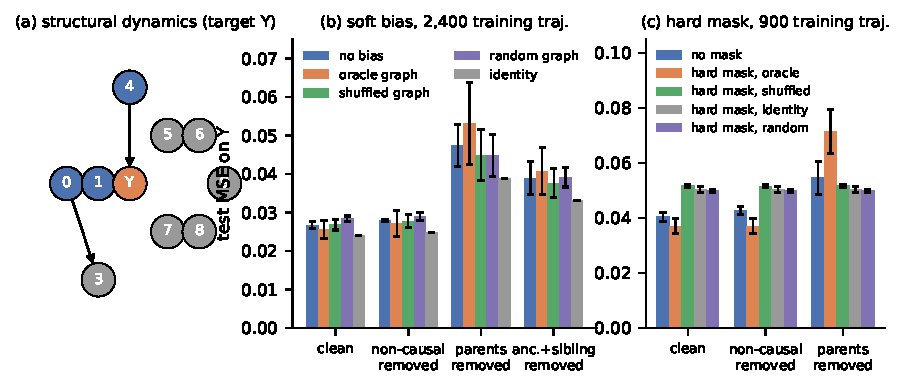
\includegraphics[width=\linewidth]{figures/fig4_structural_prior.pdf}
\caption{(a) The synthetic structural system; blue channels are ancestors of the target $Y$, grey channels cannot
influence it. (b) With 2{,}400 training trajectories, test error on $Y$ when specific channels are removed from the
test inputs, for soft attention biases built from different graphs (3 seeds; identity: 1 seed): the oracle graph
is not distinguishable from wrong or empty structure. (c) With 900 training trajectories and hard attention masks
(3 seeds): only the oracle mask improves on the unconstrained encoder, and it is the only one that depends on
$Y$'s parents.}
\label{fig:structure}
\end{figure}

\section{Analysis}
\label{sec:analysis}
\paragraph{Cost.}
Sampling-process augmentation with two views costs $1.6\times$ the time per epoch and $1.7\times$ the peak memory
of standard training ($25\to40$\,s, $3.7\to6.2$\,GB) and nothing at inference. Observation-aware queries add
$4.7$k parameters ($3.6\%$) and no measurable time. The structural bias adds no parameters (soft/hard) or $N^2$
(learned). Inference cost is $0.63$\,ms per series for every forecasting configuration.

\paragraph{Optimization plateaus with structural biases.}
On the synthetic system, several runs with an attention bias (three of nine biased full-data runs, and most
low-data runs of every configuration) stalled for their first 10--30 epochs on a constant-predictor plateau and
were terminated by patience-based early stopping, while unbiased full-data runs never did. A minimum-epoch
guard of 60 epochs let every such run escape the plateau at the default learning rate. All reported synthetic
numbers use runs that escaped; the plateau itself is a cost of the bias that a fair comparison has to account
for.

\paragraph{What the negative results say.}
The two negative findings share a theme. Cross-view consistency and structural attention priors both encode a
prior belief about what the representation should look like; both were satisfied by the optimizer in a way that
did not deliver the intended property (invariance to the observation process; reliance on true causes). The two
positive findings, augmentation and observation-aware adaptation, instead change what the model is \emph{shown}
or \emph{told} about the observation process and leave the representation free. We take this as weak evidence
that, for observation-process robustness, informing the model is more reliable than constraining it.

\paragraph{Limitations.}
All PhysioNet results use a reduced training budget and two or three seeds; ablations and classification use a
single seed or split. The forecasting study uses one dataset and one backbone. The synthetic structural system has
lagged, additive dependencies only, no confounding and no interventions, and its size makes the structure
learnable without a prior. The observation views are synthetic re-observations of real trajectories; a shift
between two real acquisition environments would be the stronger test. The PhysioNet prior is a language-model
elicitation and is evaluated only against its own permutations.

\section{Conclusion}
We have argued that irregularly sampled time series should be understood as the product of an underlying process
and an observation process, that the latter can shift independently of the former, and that this shift is a large
and under-measured failure mode for irregular time-series encoders. Of the mechanisms we studied, randomizing the
observation process during training is the most reliable remedy and transfers to unseen regimes; conditioning the
encoder on observation statistics recovers part of the effect without augmentation; enforcing representation
identity across observation views does not help and moves representations toward collapse; and supplying
variable-level structure as a soft attention prior yields in-distribution gains that a shuffled or edge-free
structure reproduces. Structural information became useful in exactly one setting: imposed as a hard constraint
when the data were too scarce to learn the structure from, where the correct graph beat every incorrect graph
of the same shape on every seed. On real clinical data a language-model-elicited physiological prior gave no
benefit. Whether an estimated or validated structure can reproduce the low-data effect on real data is the open
question we leave for future work.

\bibliographystyle{ACM-Reference-Format}
\bibliography{refs}

\end{document}
